\section{Modello di sviluppo}
La scelta del modello di sviluppo\glosp è una delle realtà fondamentali per la realizzazione di un progetto software.
Avendo una visione abbastanza chiara dell'intero progetto e, allo stesso tempo, una limitata conoscenza dei requisiti specifici, si è scelto di seguire il \textbf{modello incrementale}.

\begin{figure}[H]
	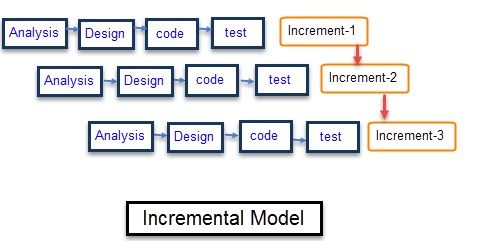
\includegraphics[width=0.99\linewidth]{res/images/incremental_model.jpg}
	\caption{Modello di sviluppo incrementale}
\end{figure}

\subsection{Modello incrementale}
Il modello di sviluppo incrementale permette la suddivisione del progetto in più sottoinsiemi,
ognuno dei quali incorpora una funzionalità diversa che, se necessario, verrà migliorata ad ogni incremento dell'intero 
sistema.  \\
Ad ogni incremento del sistema è consentita la modifica, aggiunta ed eliminazione di requisiti in base alle esigenze progettuali; 
è necessario un colloquio diretto con il proponente per approvare tali cambiamenti. \\
Utilizzando questo modello di sviluppo il versionamento del sistema è reso semplice e intuitivo, in quanto ogni modifica è facilmente tracciabile da un incremento all'altro e se ne possono valutare direttamente i difetti o benefici.\\
I vantaggi predisposti dal modello incrementale sono i seguenti:
\begin{itemize}
	\item gli incrementi sono disposti in base alle funzionalità con priorità decrescente, partendo da quelle con priorità e impatto maggiori
	così da avere subito un riscontro diretto;
	\item ogni incremento genera un risultato che può essere valutato dal proponente, approvandone i benefici o evidenziandone i difetti;
	\item rende sempre disponibile una recente baseline\glosp per una eventuale rivalutazione, senza dover ripercorrere tutti i passi effettuati fino ad ora dall'inizio dello sviluppo;
	\item tutti gli errori sono limitati al singolo incremento;
	\item le modifiche e le correzioni sono molto economiche in quanto di facile reperibilità;
	\item le fasi di test sono mirate al corrente incremento quindi più efficienti.
\end{itemize}
Sono presenti anche degli aspetti negativi per quanto riguarda il modello incrementale. La suddivisione di un singolo problema in più parti, dove almeno una di esse richiede una modifica, comporta una nuova elaborazione anche delle altre parti che non sono direttamente coinvolte, ciò aumenta in modo considerevole i tempi di sviluppo.
I problemi potrebbero derivare anche dall'architettura del sistema, la quale potrebbe non riuscire a soddisfare tutti i requisiti raccolti in anticipo per l'intero ciclo di vita del software.


